\section{Introduzione}

\textcolor{red}{PARLA DEL CITOMETRO IN GENERALE E DEL PERCHè USARE L'APPROCCIO ECM}

\textcolor{blue}{\lipsum[1]}

\section{Background}

\begin{figure*}[h!]
	\begin{subfigure}{0.5\linewidth}
			\centering
				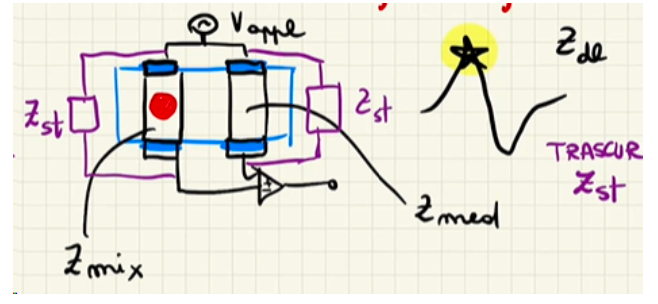
\includegraphics[width=0.95\linewidth]{figures/modello_circuitale}
				\caption{}
	\end{subfigure}\hfill
	\begin{subfigure}{0.5\linewidth}
	\centering
	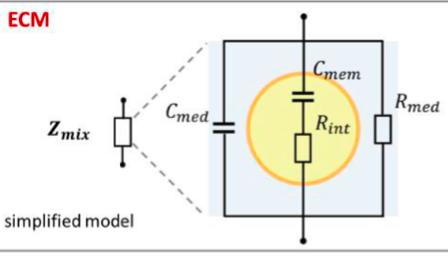
\includegraphics[width=0.5\linewidth]{figures/modello_circuitale1}
	\caption{}
\end{subfigure}\hfill
	\caption{Schema circuitale di misura nel citometro ad impedenza e tipico segnale (a); equivalente circuitale per cellula nel mezzo. Il segnale bipolare presenta il picco nel momento in cui la cellula passa tra le coppie parallele di elettrodi. Nello schema circuitale sono trascurate eventuali impedenze parassite.}
	\label{fig:modellocircuitale}
\end{figure*}



La modellazione tramite equivalente circuitale porta in contro la teoria delle miscele di Maxwell (MMT) per modellare le proprietà dielettriche cellulari.

Tale modello permette di descrivere il segnale ottenuto in un citometro ad impedenza ad elettrodi paralleli nel momento in cui la cellula si trova tra una coppia di elettrodi. La presenza della cellula tra gli elettrodi, insieme alla perturbazione del campo elettrico, genera un segnale di corrente differenziale che risulta proporzionale al diametro per il tramite del fattore di Clausis-Mossotti \cite{bibid}.

Nel seguente report verrà considerata una versione semplificata del segnale, pari a:

\begin{equation}
	S=r^{3} f_{C M}
\end{equation}

\subsection{Equivalenza circuitale}

Il circuito in \cref{fig:modellocircuitale} prevede l'applicazione di un potenziale agli elettrodi superiori e il campionamento del segnale dagli elettrodi inferiori, come corrente differenziale.

Osservando il percorso della corrente essa si troverà a passare per gli elettrodi e poi per il buffer conduttivo, eventualmente anche incontrando la cellula. Ognuno di questi materiali contribuirà con una sua impedenza.

Tali impedenze sono in serie e quindi il segnale misurato sarà:

\begin{equation}
	I_{\operatorname{d i f f}}=\frac{V_{\operatorname{a p p l}}}{Z_{\operatorname{m e d}}+2 Z_{d l}}-\frac{V_{\operatorname{a p p l}}}{Z_{\operatorname{m i x}}+2 Z_{d l}}
\end{equation}

Dove l'impedenza $Z_{\operatorname{m i x}}$ rappresenta l'insieme di cellula e buffer conduttivo e verrà descritta più avanti tramite MMT.

Inoltre, in questo segnale, riorganizzando i termini, compare una differenza di impedenza $\Delta Z=Z_{\operatorname{m i x}}-Z_{\operatorname{m e d}}$ pari proprio alla perturbazione indotta dalla cellula.  Tale termine inoltre risulta molto minore dell'impedenza del mezzo e questo ci permette di trascurare i termini quadratici e ottenere un segnale di corrente differenziale pari a:

\begin{equation}
	I_{\operatorname{d i f f}}\approx {V_{\operatorname{a p p l}}\over Z_{\operatorname{m e d}}^2} \frac{Z_{\operatorname{m i x}} -Z_{\operatorname{m e d}}}{\left(1+ 2{Z_{dl}\over Z_{\operatorname{m e d}} }\right)^2}
	\label{eq:idiff}
\end{equation}

L'impedenza di elettrodo è legata alla capacità superficiale $C_{dl}$ e alle dimensioni del volume del canale compreso tra le coppie. Risulta essere pari a:

\begin{equation}
	Z_{d l}=\frac{1}{j \omega C_{d l} w l}
\end{equation}

L'impedenza del mezzo viene espressa tramite la legge di Ohm, contestualizzandola in funzione del volume del canale:

\begin{equation}
	Z_{\operatorname{m e d}}=\frac{h}{\sigma^{*} l w k}={1\over \sigma^*}{1\over G}={1\over j\omega \varepsilon ^*}{1\over G}
\end{equation}

Portando in conto anche effetti di distorsione del campo elettrico tramite un coefficiente geometrico $G$. 

In generale, la permittività complessa è esprimibile come:

\begin{equation}
	\varepsilon^{*}=\varepsilon+\frac{\sigma}{j \omega}
\end{equation}

Tali considerazioni sono analoghe per l'impedenza del mix dove però la $\varepsilon^*_{\operatorname{m i x}}$ va stimata tramite la teoria delle miscele di Maxwell. 

\subsection{Maxwell's Mixtures theory}

La teoria delle miscele di Maxwell permette di descrivere la permettività complessa di mezzo e cellula in funzione delle loro proprietà.

In particolare, si può esprimere la permettività in funzione del fattore di Clausius-Mossotti come:

\begin{equation}
	\varepsilon_{\operatorname{mix}}^{*}=\varepsilon_{\operatorname{m e d}}^{*} \frac{1+2 \varphi f_{C M}}{1-\varphi f_{C M}}
\end{equation}

A sua volta questo fattore si esprime in funzione delle proprietà della cellula:

\begin{equation}
	f_{C M}=\frac{\varepsilon_{\operatorname{c e l l}}^{*}-\varepsilon_{\operatorname{m e d}}^{*}}{\varepsilon_{\operatorname{c e l l}}^{*}+2 \varepsilon_{\operatorname{m e d}}^{*}}
\end{equation}

Mettendo insieme quanto descritto si ottiene l'espressione per la corrente differenziale in \cref{eq:idiff}, in funzione del fattore di Clausius-Mossotti:

\begin{equation}
	I_{d i f f} \approx-\frac{V_{\operatorname{a p p l}}}{Z_{\operatorname{m e d}}} \frac{1}{\left[1+\frac{2 Z_{d l}}{Z_{\operatorname{m e d}}}\right]^{2}} 3 \varphi f_{CM}
\end{equation}

Dove $\varphi$ è la volume fraction che porta in conto il volume della cellula come:

\begin{equation}
	\varphi=\frac{V_{\text {cell }}}{V_{\text {misura }}}=\frac{\frac{4 \pi r^{3}}{3}}{l w h K}
\end{equation}

E il segnale misurato, trascurando i contributi dispersivi legati agli elettrodi, risulta proporzionale a $r^3$ (tramite la volume fraction) e al fattore di Clausius-Mossotti.


\begin{figure}[h!]
	\centering
	
\includegraphics[width=0.7\linewidth]{figures/screenshot001}
	\caption{SINGLE SHELL VS DOUBLE SHELL. 3/4 dell'immagine per spiegare l'0omogenizzazione double}
	\label{fig:screenshot001}
\end{figure}


\subsection{Shell model}

Avendo visto come portare in conto le proprietà miste di cellula e mezzo non rimane che analizzare come omogeneizzare le proprietà della singola cellula. 
Le cellule vengono omogenizzate ad un unico materiale avente proprietà $\varepsilon^*_{\operatorname{cell}}$ e tale da portare in conto sia le proprietà della parte interna che della membrana cellula.

Per cellule prive di nucleo, come i globuli rossi, è possibile utilizzare un modello \textbf{single shell}, basato quindi su una membrana esterna sottile ed una zona interna le cui proprietà vengono omogeneizzate come:

\begin{equation}
	\varepsilon_{c e l l}^{*} \approx \varepsilon_{i n t}^{*} \frac{\chi}{1+\chi}
	\label{eq:shell}
\end{equation}

Dove:

\begin{equation}
	\chi=\frac{\varepsilon_{m e m}^{*} / d_{m e m}}{\varepsilon_{i n t}^{*} / r}
\end{equation}

Per cellule più grandi e complesse è necessario considerare un modello più accurato come il \textbf{double shell} dove vengono considerate quattro differenti zone. Si considera una zona interna, corrispondente al nucleo, ($\operatorname{np}$) e la sua membrana $\operatorname{ne}$. A queste si aggiunge il citoplasma $\operatorname{cyt}$ e la membrana cellulare $\operatorname{mem}$. 

In particolare, si effettuano delle omogenizzazioni in sequenza partendo dalla zona centrale. 

Applicando una relazione analoga a \cref{eq:shell} si arriva a stimare le proprietà complessive del nucleo ($\operatorname{nuc}$). Successivamente queste possono essere unite proprio tramite la MMT descrivendo così l'interno cellulare ($\operatorname{int}$). Infine, si ripete l'omogenizzazione (\cref{eq:shell}) tra la zona interna e la membrana ottenendo così una permittività complessa per l'intera cellula. 

\textcolor{red}{PARLA DELL?UTILIT° per separare le cellule LOL}

\section{Risultati}

Vengono quindi applicati questi modelli per modellare segnali di citometria ad impedenza di diverse cellula vitali, necrotiche e apoptotiche \cite{de_ninno_high-throughput_2020}.




\textcolor{blue}{\lipsum[1-4]}





\section{Conclusioni}

\textcolor{blue}{\lipsum[1-2]}


\raggedbottom


\raggedbottom
\pagebreak
\section*{Disponiblità dei dati}

Il materiale è disponibile alla repository online del progetto: \url{https://github.com/mastroalex/ecm-mmt}.

\printbibliography[title=Riferimenti]
%\section*{References}

\clearpage
\onecolumn
\section*{Appendice}

